\documentclass[tikz]{standalone}
\usepackage{tikz}
\usepackage{amssymb}
\usetikzlibrary{positioning}
\usetikzlibrary{calc}
\usetikzlibrary{arrows,shapes,snakes,automata,petri}
\begin{document}
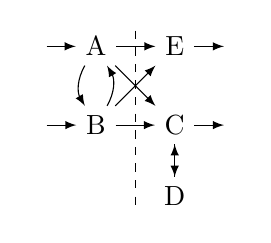
\begin{tikzpicture}
\node[](startA) at (-0.75,0){};
\node[](startB) at (-0.75,-1){};
\node[](A) at (0,0){A};
\node[](B) at (0,-1){B};
\node[](C) at (1,-1){C};
\node[](D) at (1,-1.9){D};
\node[](E) at (1,0){E};
\node[](endC) at (1.75,-1){};
\node[](endE) at (1.75,0){};

\draw[dashed](0.5,0.2)--(0.5,-2.1);

\path
(startA) edge[-latex]node{} (A)
(startB) edge[-latex]node{} (B)
(A) edge[-latex, bend right]node{} (B)
(B) edge[-latex, bend right]node{} (A)
(A) edge[-latex]node{} (E)
(A) edge[-latex]node{} (C)
(B) edge[-latex]node{} (E)
(B) edge[-latex]node{} (C)
(C) edge[-latex]node{} (D)
(D) edge[-latex]node{} (C)
(C) edge[-latex]node{} (endC)
(E) edge[-latex]node{} (endE);
\end{tikzpicture}
\end{document}